\section{Formatting}  

A thesis is written with a single-column layout on one- or two-sided
A4 sheets. The font type of the body text is usually Times New Roman 
and the font size is 12 pt. The text is fully justified and hyphenated.
You do not have to indent the paragraphs.

\subsection{Mathematical notations}

Numbers are generally written using numerals for the sake of clarity,
for example ``6 stages'' rather than ``six stages''. You should
also use a thousand separators\footnote{Use tilde \~{} in LaTeX and a
  special character \textit{non-breaking space} in MS Word},
i.e. instead of 55700125 write 55~700~125. Never omit the leading zero
in decimals. For example, it is correct to write ``0.5'' and wrong to
write ``.5''. A comma is used as a decimal separator in the Estonian
language and a period in the English language.

Like numbers, it is advisable to abbreviate units of
measurement. There is a space between the number and the unit, but you
should keep them on the same line. It is better to compile a table or
graph than include a great deal of numerical values in the body
text. Use precise language and put numbers on a scale.

Newton's Second Law can be presented in the following way:

\begin{equation}
  \label{eq:newton2}
 ma= F,
\end{equation}

where $m$ denotes the mass of an object, $a$ means acceleration, and
$F$ means force. Please note that all the variables must be defined at
the point of their first appearance. All sentences end with a
punctuation mark, and the main elements of a sentence are separated by
a comma in accordance with the rules of English grammar. Consider formulas 
as part of a sentence, therefore use commas or period accordingly after 
formulas (e.g. see equation (\ref{eq:newton2})).

Formulas can be numbered or not numbered. Numbered formulas are used if there is need to refer to these formulas later on. For example, let us have a formula
\begin{equation}\label{eq:pythagoras}
c^2=a^2+b^2.
\end{equation}
Then, since \eqref{eq:pythagoras} is numbered, we can always refer to it in later text. For example, specifying $a=3$ and $b=4$ and applying \eqref{eq:pythagoras} implies $c=5$.

On the other hand, if we do not refer to some formula or equation at all, it should not have a number, for example:
\[
S_n=\sum_{i=1}^n X_n.
\]

Occasionally mathematical notations are preceded by an
identifier, such as 'Definition 1' or 'Theorem 1'. Simple formulas may 
be displayed within the body of the text without numbering.

Please note that usually different styles applied to same letter/symbol refer to different object, for example, $x$, x, $X$, \textit{\textbf{X}}, $\mathbf{X}$, ..., are all different. Also, a general rule is that variables are in italic and function names are in regular font, for example, $s$, $u$ and $p$ are some variables, and supremum function $\sup$ is in regular font so we do not confuse it with the product $sup=s\cdot u\cdot p$. 

Please try to use unified notation (i.e. same letter/symbol should mean the same variable or function) throughout the whole document (as much as possible).


LaTeX is the best editor for writing also the more complex equations, such as
\begin{equation}
  \label{eq:fourier}
  G^+(t,t')= \int G^+(E) exp[-iE(t-t')/\hbar] dE.
\end{equation}


\subsection{Figures}

You must refer to all the figures in the body text. The reference
should preferably appear on the same page as the actual figure or
before it (e.g. Figure~\ref{fig:ex_fig}). Figures and tables must be numbered consistently thesis
and primarily placed at the top of the page, but you are free to
decide where they fit best. Never start a chapter with a figure, table
or list.
% Note: put tilde between text and ref command, like in
% 'Figure~\ref{fig:ex_fig}' above. Tilde (~) puts a white space but
% prevents line break. Same thing applies to Table~\ref{tab:summary}
% as well.

Figures and the caption are consistently centered  and the caption is 
placed under the figure and always on the same page as the figure. 
All figures must be explained in the body text, so that readers know 
what they are supposed to notice. 

The figures should be in the same language as other text. The recommended 
font size is the same as that of the body text but no smaller than 10 pt. 
The figures must be readable, even if your thesis is printed in grey-scale!

% Here's an example how to add a figure. Default placement of figures
% is at top of page, i.e. placement specifier is '[t]' could be
% omitted.  The dimensions can be relative to text width (or height)
% or absolute (4 cm).

\begin{figure}[t]
  \begin{center}
    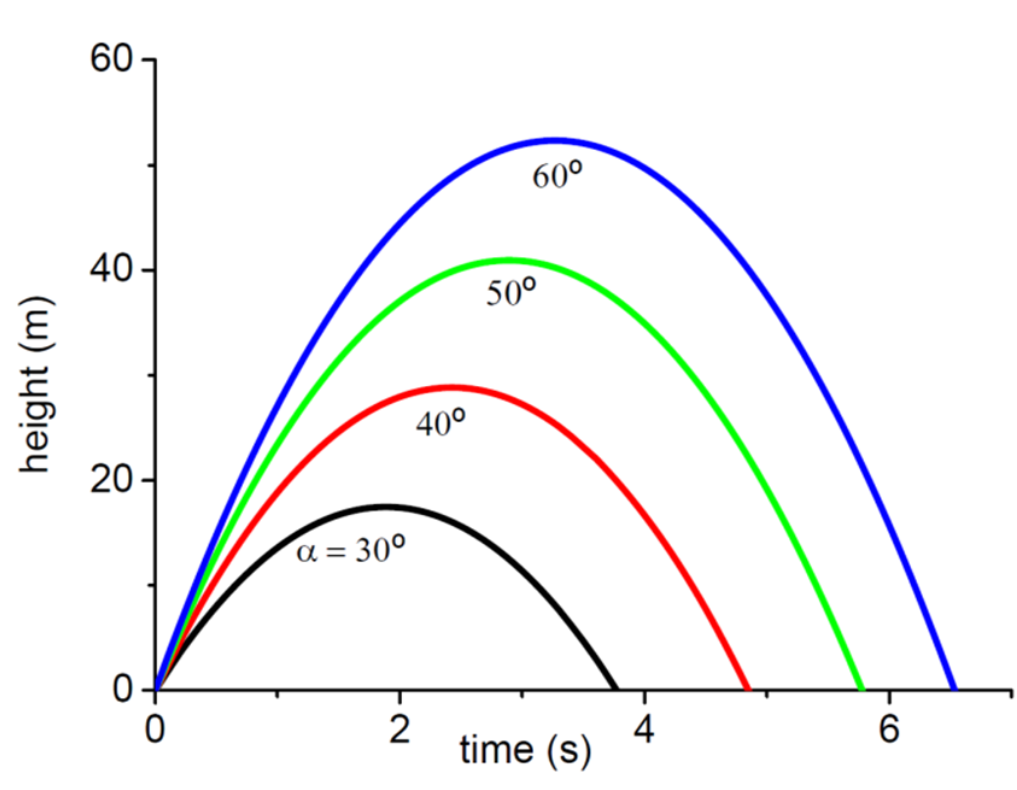
\includegraphics[width=0.7\textwidth]{figure}
  \end{center}
  \caption{Diagram of achieved height and time of flight with different angles of release.}
  \label{fig:ex_fig}
\end{figure}


\subsection{Tables}

Tables have numbered captions, see Table\ref{tab:thin_film} for
example. The caption is placed on the same page above the table. You 
must refer to all the tables in the body text. In addition, you must 
discuss the content of any tables in the body text to ensure that readers 
understand their relevance.

\begin{table}[ht]
  \small
  \begin{center}
    \caption{Example of evaporation conditions in a thin film structure.}
    \label{tab:thin_film}
    \begin{tabular}{l | r r r r r r}
      % l = align to left (e.g. text), c=align to center, r=align to
      % right (e.g. numbers), Pipe | creates vertical line
      % Let's put 1 horinzontal line above the table, 2 after header rows,  and 1 below
      \hline
      \textbf{Substance} & \textbf{Thickness}& \textbf{Correction } & \textbf{Pressure} & \textbf{Temper-}          & \textbf{Current} & \textbf{Speed} \\
                         & \textbf{(nm)}     & \textbf{coefficient} & \textbf{(mbar)}   & \textbf{ature ($^\circ$C)} & \textbf{(mA)}    & \textbf{(nm/s)} \\
      \hline 
      SiO2	& 181.0	& 1.10	& $3.0\cdot10^5$	& 90.6	& 20-23	 &0.2 \\
      TiO2	& 122.1	& 1.55	& $1.5\cdot10^4$	& 91.1	& 100-93 &0.1 \\
      \hline
    \end{tabular}
  \end{center}
\end{table}


Often it is better to create the table in, e.g. MS Excel, and import
it as .eps or .pdf file, for example, when you calculate some of the
values automatically.
%\begin{table}[h]
%  \begin{center}
%    \caption{Example of evaporation conditions in a thin film structure.}
%    \label{tab:thin_film_graphics}
%    \includegraphics[width=8cm]{my_table.eps}
%  \end{center}
%\end{table}

You can use boldface to highlight the header row. Do not surround all 
the cells with a border, as it may make your table harder to read. 
Put a line on top and bottom of the table. You can add a horizontal line
grouped into categories.

The numbers are right aligned (optimally lined up at the decimal
point) for easy comparison. You should preferably use SI units,
established prefixes and rewrite large numbers so that the power of
ten should be placed in the title of the column instead of each row,
if possible. 


\subsection{Programs and algorithms}

Codes and algorithms are written using mono-spaced font, such as
Courier New, Consolas or their variations. If the length of the code
or algorithm is less than 10 lines and you do not refer to it later on
in the text, you can present it similarly to formulas.  Here's an
example showing a snippet:

\begin{lstlisting}[style=console, % title={Template files} ] 
all: ${TARGET}.tex
	pdflatex ${TARGET}.tex
	bibtex ${TARGET}
	pdflatex ${TARGET}.tex
\end{lstlisting}  

If the code is longer but shorter than a page, you present like a
figure (Program 4.1) titled ``Program'' or ``Algorithm''.
You should add some comments to the code and indent it
consistently. The actions performed by the code must be outlined in
broad terms in the body text. Line numbers make it much easier to
refer to the code in the text. 

LaTeX has a packages that enable automatic code formatting like
highlight reserved words, bring out string input or color comments differently.